\documentclass[12pt]{article}
\usepackage[utf8]{inputenc}
\usepackage[a4paper, total={6.5in, 9.5in}]{geometry}
\usepackage{authblk}
\usepackage{multirow}
\usepackage{graphicx}
\usepackage{amsmath}
\usepackage{biblatex}
\usepackage{rotating}
\usepackage{ragged2e}
\usepackage{multicol}
\usepackage{float}
\usepackage{algpseudocode}
\usepackage{enumitem}
\usepackage{caption}
\usepackage{subcaption}
\usepackage{hyperref}
\hypersetup{
    colorlinks=true,
    linkcolor=blue,
    }
\usepackage[label=corner]{karnaugh-map}
\usepackage[siunitx, RPvoltages]{circuitikz}
\usetikzlibrary{calc}
\usepackage{tikz}
\usetikzlibrary{positioning, shapes, arrows.meta, calc}

\title{CSE 306 \\
Computer Architecture Sessional \\
\vspace{10mm}
Assignment-3: 8-bit MIPS Design, Simulation, and Implementation \\
\vspace{20mm}
Section - A1 \\
Group - 01 \\
\vspace{15mm}
\RaggedRight
Members of the Group: \\
\normalsize	{
\begin{enumerate}[label=\roman*]
    \item 1905001 - Mohammad Sadat Hossain
    \item 1905002 - Nafis Tahmid
    \item 1905004 - Asif Azad
    \item 1905005 - Md. Ashrafur Rahman Khan
    \item 1905008 - Shattik Islam Rhythm
\end{enumerate}
}
}
\author{}
\date{}

\begin{document}
\maketitle
\newpage
\tableofcontents

\newpage
\section{\large{Introduction}}
MIPS (Microprocessor without Interlocked Pipeline Stages) is a Reduced Instruction Set Computing (RISC) architecture that has been widely used in the design of microprocessors and embedded systems due to its simplicity, efficiency, and flexibility. In this report, we present the design and implementation of an 8-bit MIPS PC with pipelining, which is a technique used to increase the throughput of a processor by overlapping the execution of multiple instructions.\\

The pipelining technique is based on the observation that most instructions in a program can be broken down into a series of smaller and simpler operations that can be executed independently and in parallel. By dividing the processor into several stages, each responsible for one of these operations, instructions can be processed simultaneously, resulting in a significant improvement in performance.\\

The design of our MIPS computer is based on the five-stage pipeline architecture commonly used in modern processors, which consists of the following stages: instruction fetch, instruction decode, execution, memory and write back. Since the last stage does not require any significantly new hardware, it can be merged with the previous stage. Each of these stages is responsible for a specific part of the instruction processing and is connected to the next stage through a pipeline register, which holds the data until it is needed by the next stage.\\

We have created an 8-bit computer that consists of an 8-bit data bus, an 8-bit address bus, and an 8-bit Arithmetic and Logic Unit (ALU). To conform to standard design principles, we have included separate instruction and data memory in our design. 
% The instruction set supported by the computer is listed in section \ref{IS}. The complete circuit diagram is shown in section \ref{Circ}. Method of programming and execution is explained in section \ref{prog} and special features are stated in section \ref{Spec}. Lastly, in section \ref{IC}, list of ICs used is presented.

\newpage
\section{\large{Instruction Set}}
\label{IS}
\subsection{Instruction Set Description}
\begin{table}[h]
    \centering
   \begin{tabular}{|c|c|c|}
    \hline
    Instruction ID & Instruction Type & Instruction \\
    \hline
    A & Arithmetic & add \\
    \hline
    B & Arithmetic & addi \\
    \hline
    C & Arithmetic & sub \\
    \hline
    D & Arithmetic & subi \\
    \hline
    E & Logic & and \\
    \hline
    F & Logic & andi \\
    \hline
    G & Logic & or \\
    \hline
    H & Logic & ori \\
    \hline
    I & Logic & sll \\
    \hline
    J & Logic & srl \\
    \hline
    K & Logic & nor \\
    \hline
    L & Memory & lw \\
    \hline
    M & Memory & sw \\
    \hline
    N & Control & beq \\
    \hline
    O & Control & bneq \\
    \hline
    P & Control & j \\
    \hline
\end{tabular}
\caption{Instruction Set Assignment}
\end{table}

\subsection{Instruction Format}
\begin{itemize}
    \item R-type \hspace{10}
        \begin{tabular}{|p{2cm}|p{2cm}|p{4cm}|p{2.5cm}|}
        \hline
         Opcode & Src Reg 1 & Src Reg 2 & Dst Reg  \\
         \hline
         4 bits & 4 bits & 4 bits & 4 bits \\
         \hline
        \end{tabular}
    \item S-type \hspace{12}
        \begin{tabular}{|p{2cm}|p{2cm}|p{4cm}|p{2.5cm}|}
        \hline
        Opcode & Src Reg 1 & Dst Reg & Shamt  \\
        \hline
        4 bits & 4 bits & 4 bits & 4 bits \\
        \hline
        \end{tabular}
    \item I-type \hspace{14}
        \begin{tabular}{|p{2cm}|p{2cm}|p{4cm}|p{2.5cm}|}
        \hline
         Opcode & Src Reg 1 & Src Reg 2/Dst Reg & Addr./Immdt.  \\
         \hline
         4 bits & 4 bits & 4 bits & 4 bits \\
         \hline
    \end{tabular}
    \item J-type \hspace{13}
        \begin{tabular}{|p{2cm}|p{6.4cm}|p{2.5cm}|}
        \hline
         Opcode & Target Jump Address & 0  \\
         \hline
         4 bits & 8 bits & 4 bits \\
         \hline
    \end{tabular}
\end{itemize}


\newpage
\subsection{Instruction Set Assignment}
\begin{table}[h]
    \centering
    \begin{tabular}{|c|c|c|}
    \hline
    Serial Number & Instruction ID & Opcode \\
    \hline
    0 & K & 0000 \\
    \hline
    1 & J & 0001 \\
    \hline
    2 & E & 0010 \\
    \hline
    3 & I & 0011 \\
    \hline
    4 & O & 0100 \\
    \hline
    5 & P & 0101 \\
    \hline
    6 & F & 0110 \\
    \hline
    7 & D & 0111 \\
    \hline
    8 & L & 1000 \\
    \hline
    9 & M & 1001 \\
    \hline
    10 & C & 1010 \\
    \hline
    11 & B & 1011 \\
    \hline
    12 & G & 1100 \\
    \hline
    13 & N & 1101 \\
    \hline
    14 & H & 1110 \\
    \hline
    15 & A & 1111 \\
    \hline
\end{tabular}

    \caption{Instruction Set Assignment}
\end{table}


\newpage
\section{\large{Circuit Diagram}}
\label{Circ}
\begin{figure}[H]
     \centering
     
\includegraphics[width=\textwidth]{Images/Instruction Fetch.png}
     \caption{Instruction Fetch}
     \label{fig:if}
 \end{figure}

 \begin{figure}[H]
     \centering
     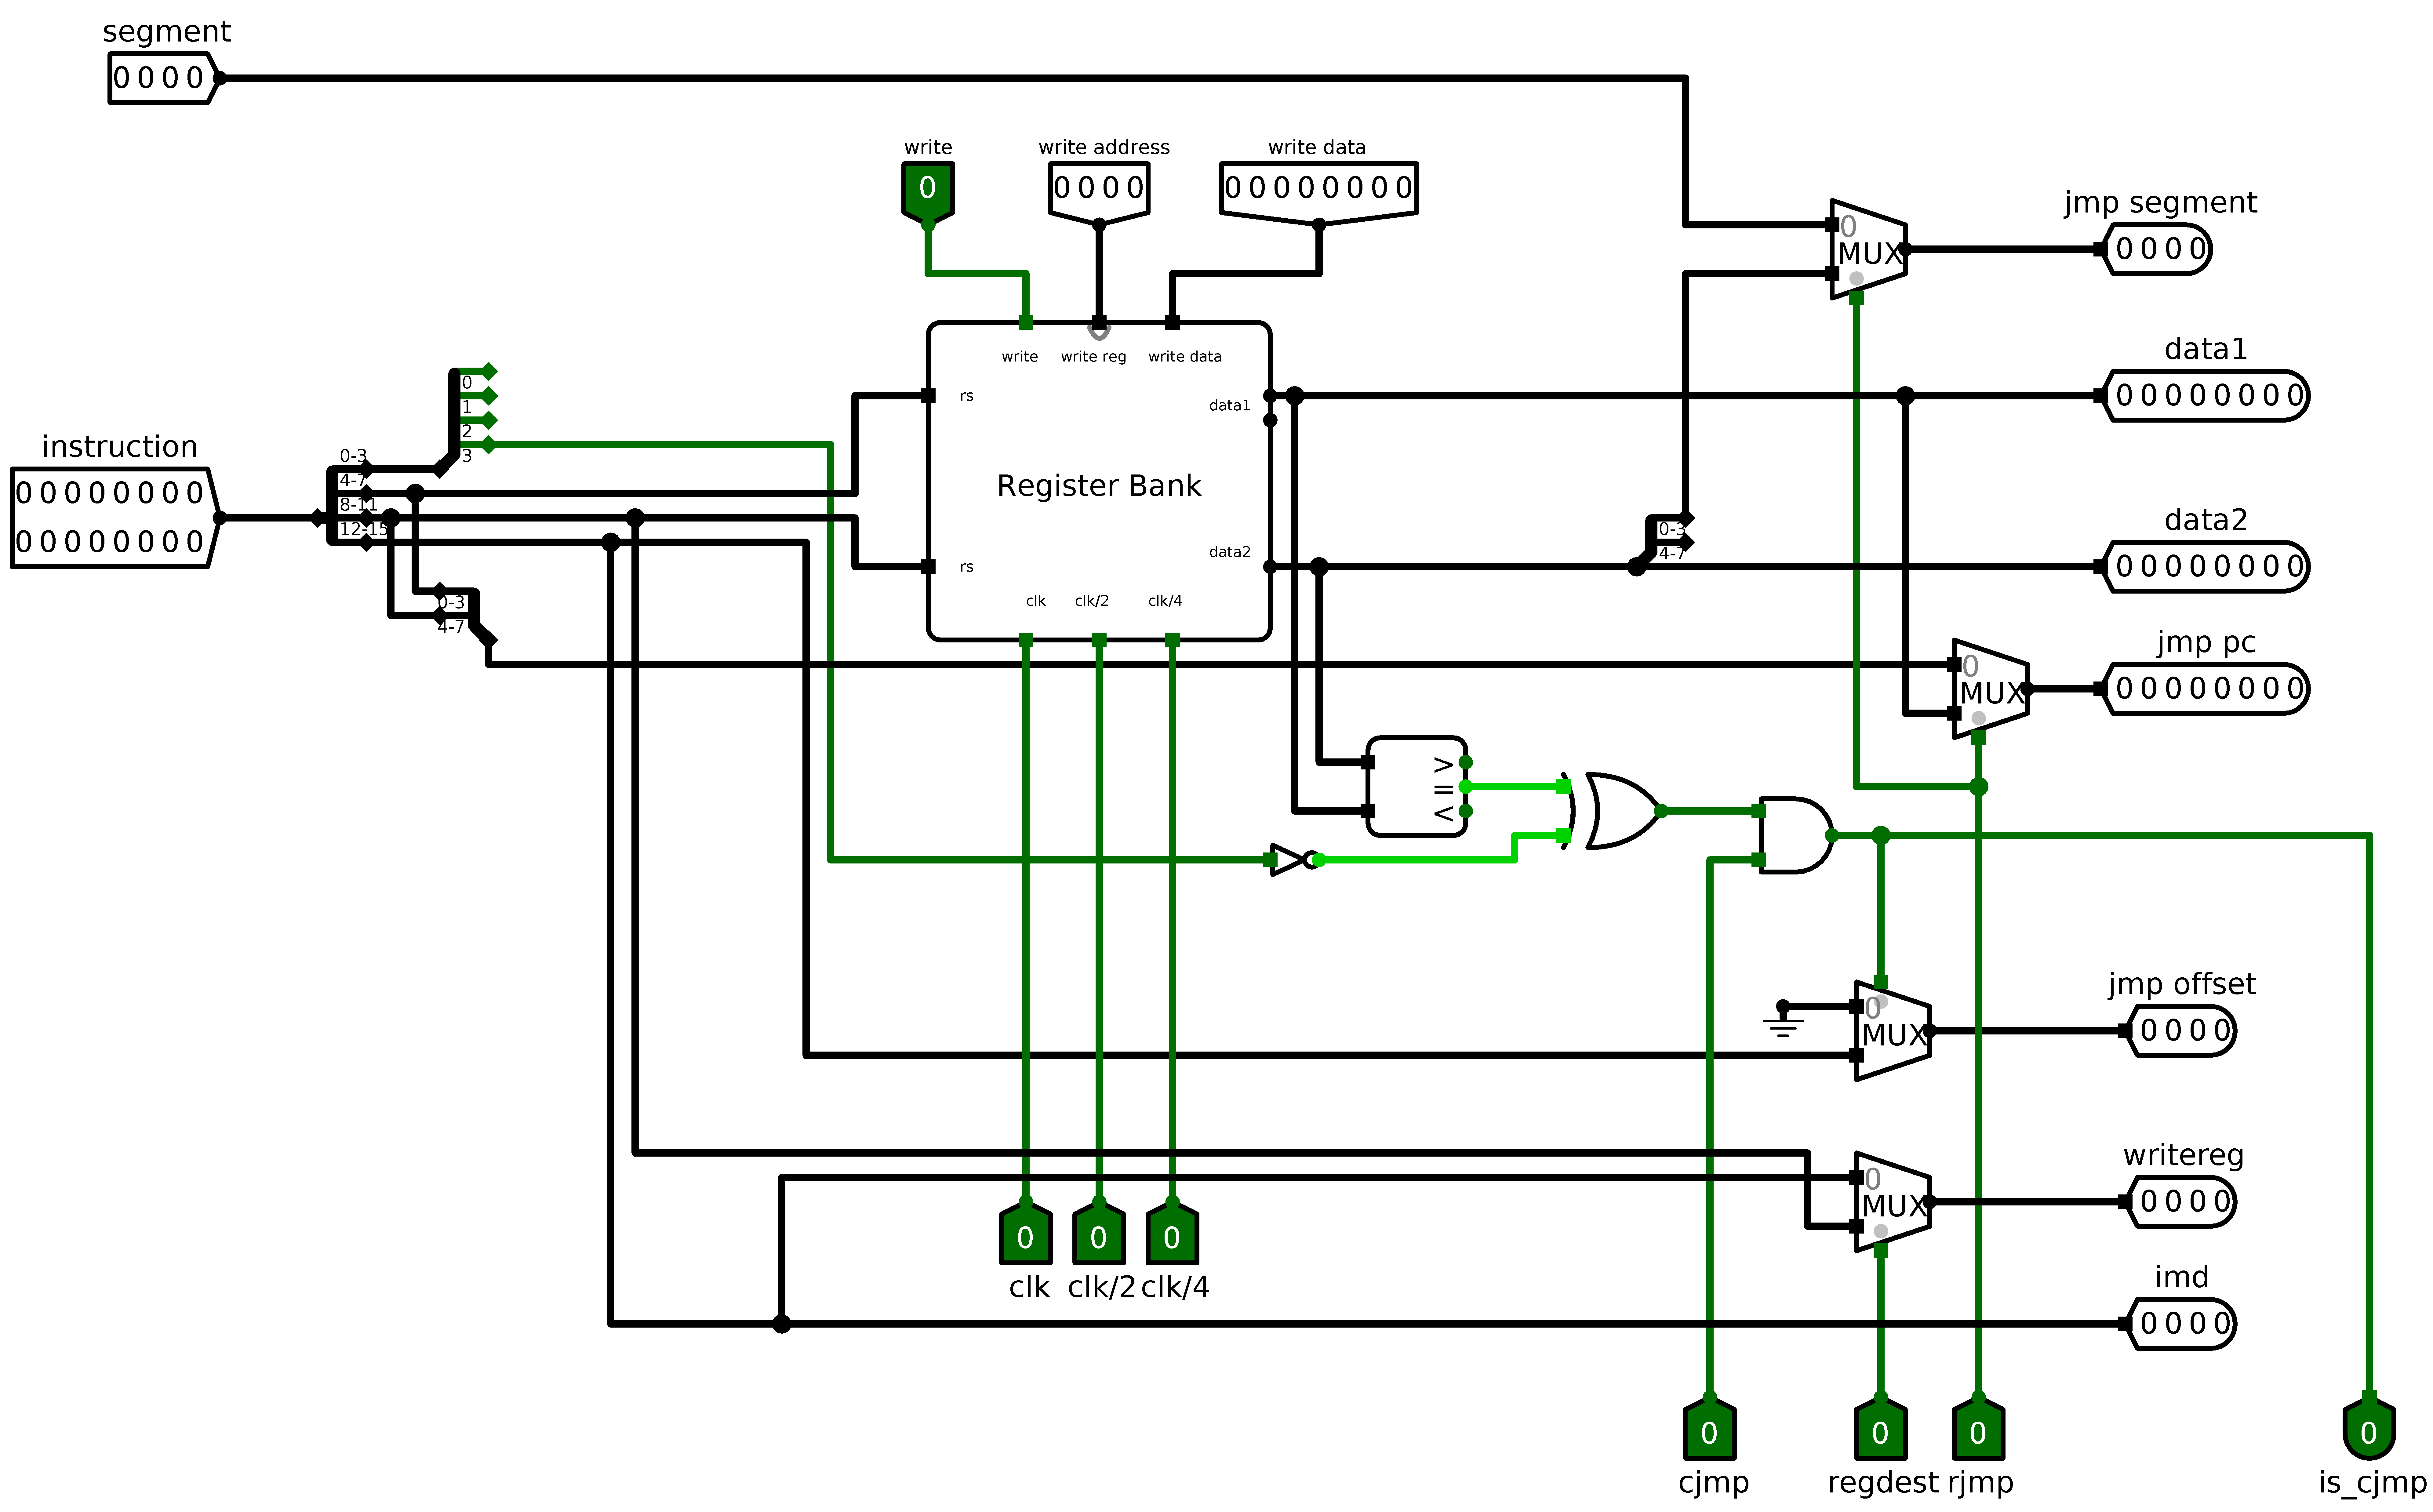
\includegraphics[width=\textwidth]{Images/Instruction Decode.png}
     \caption{Instruction Decode}
     \label{fig:id}
 \end{figure}

 % \begin{figure}[H]
 %     \centering
 %     \includegraphics[width=0.8\textwidth]{Images/PC Update.png}
 %     \caption{PC Update}
 %     \label{fig:pcu}
 % \end{figure}

 \begin{figure}[H]
     \centering
     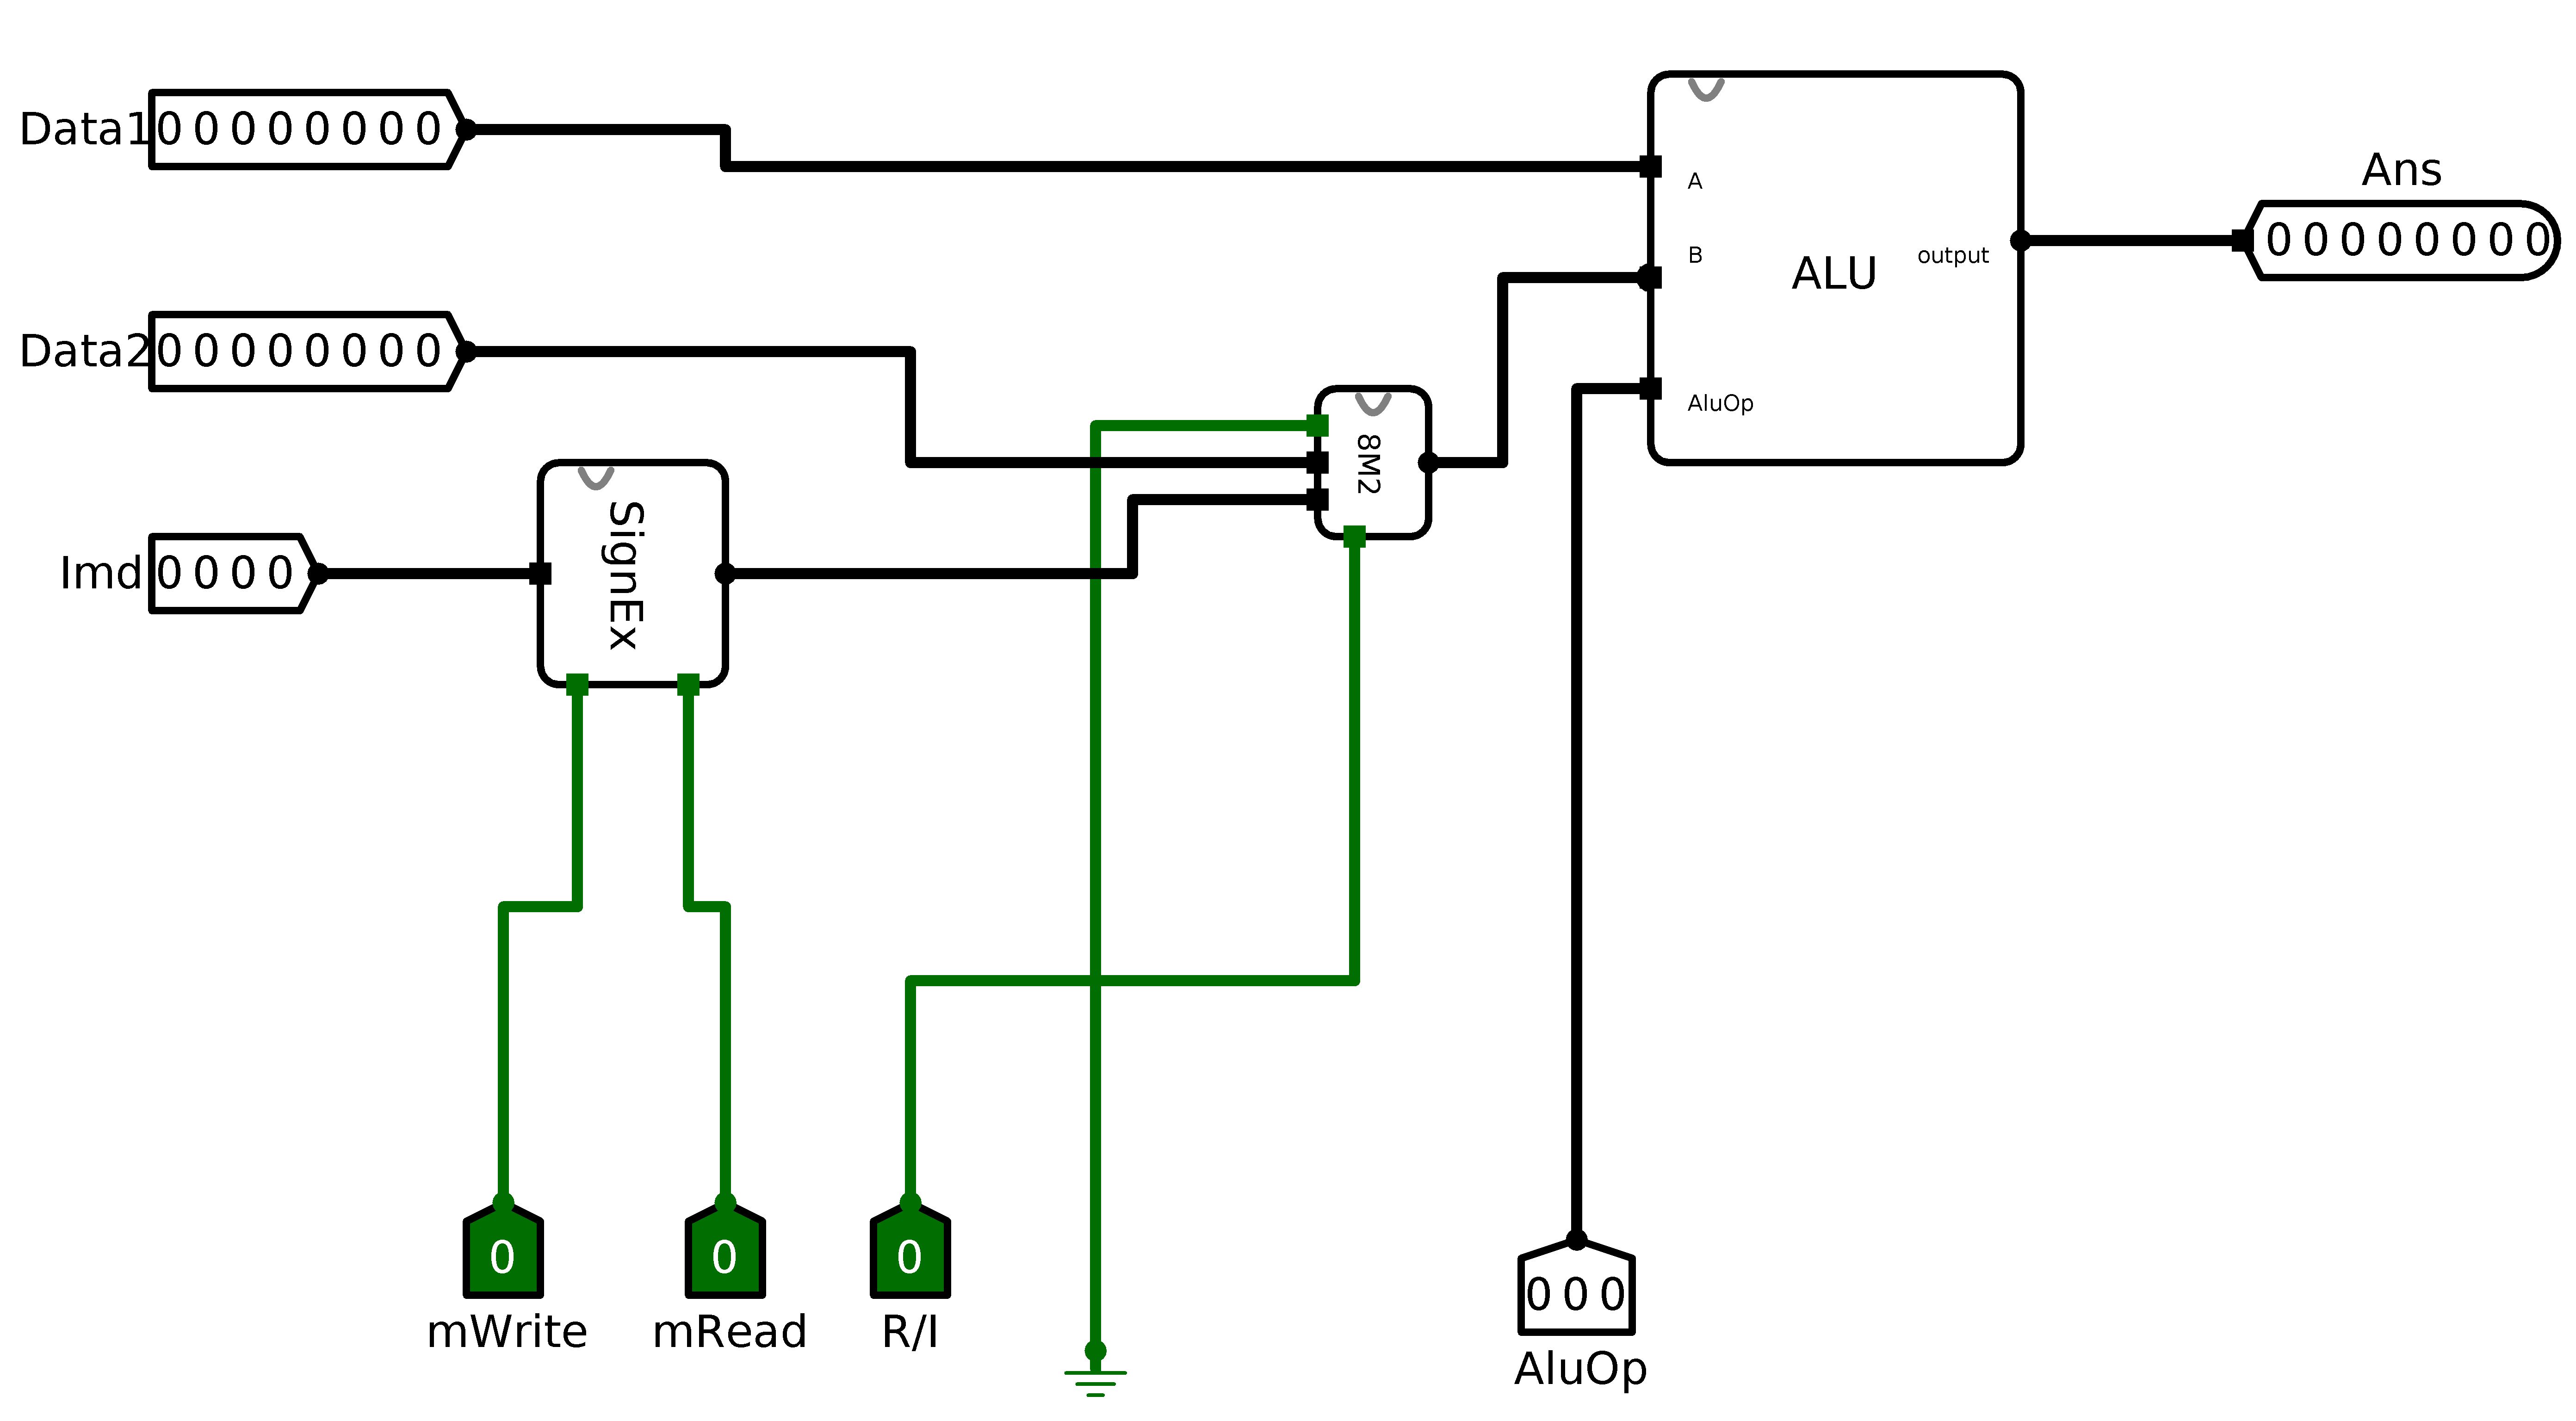
\includegraphics[width=\textwidth]{Images/Execution.png}
     \caption{Execution Unit}
     \label{fig:exec}
 \end{figure}

 \begin{figure}[H]
     \centering
     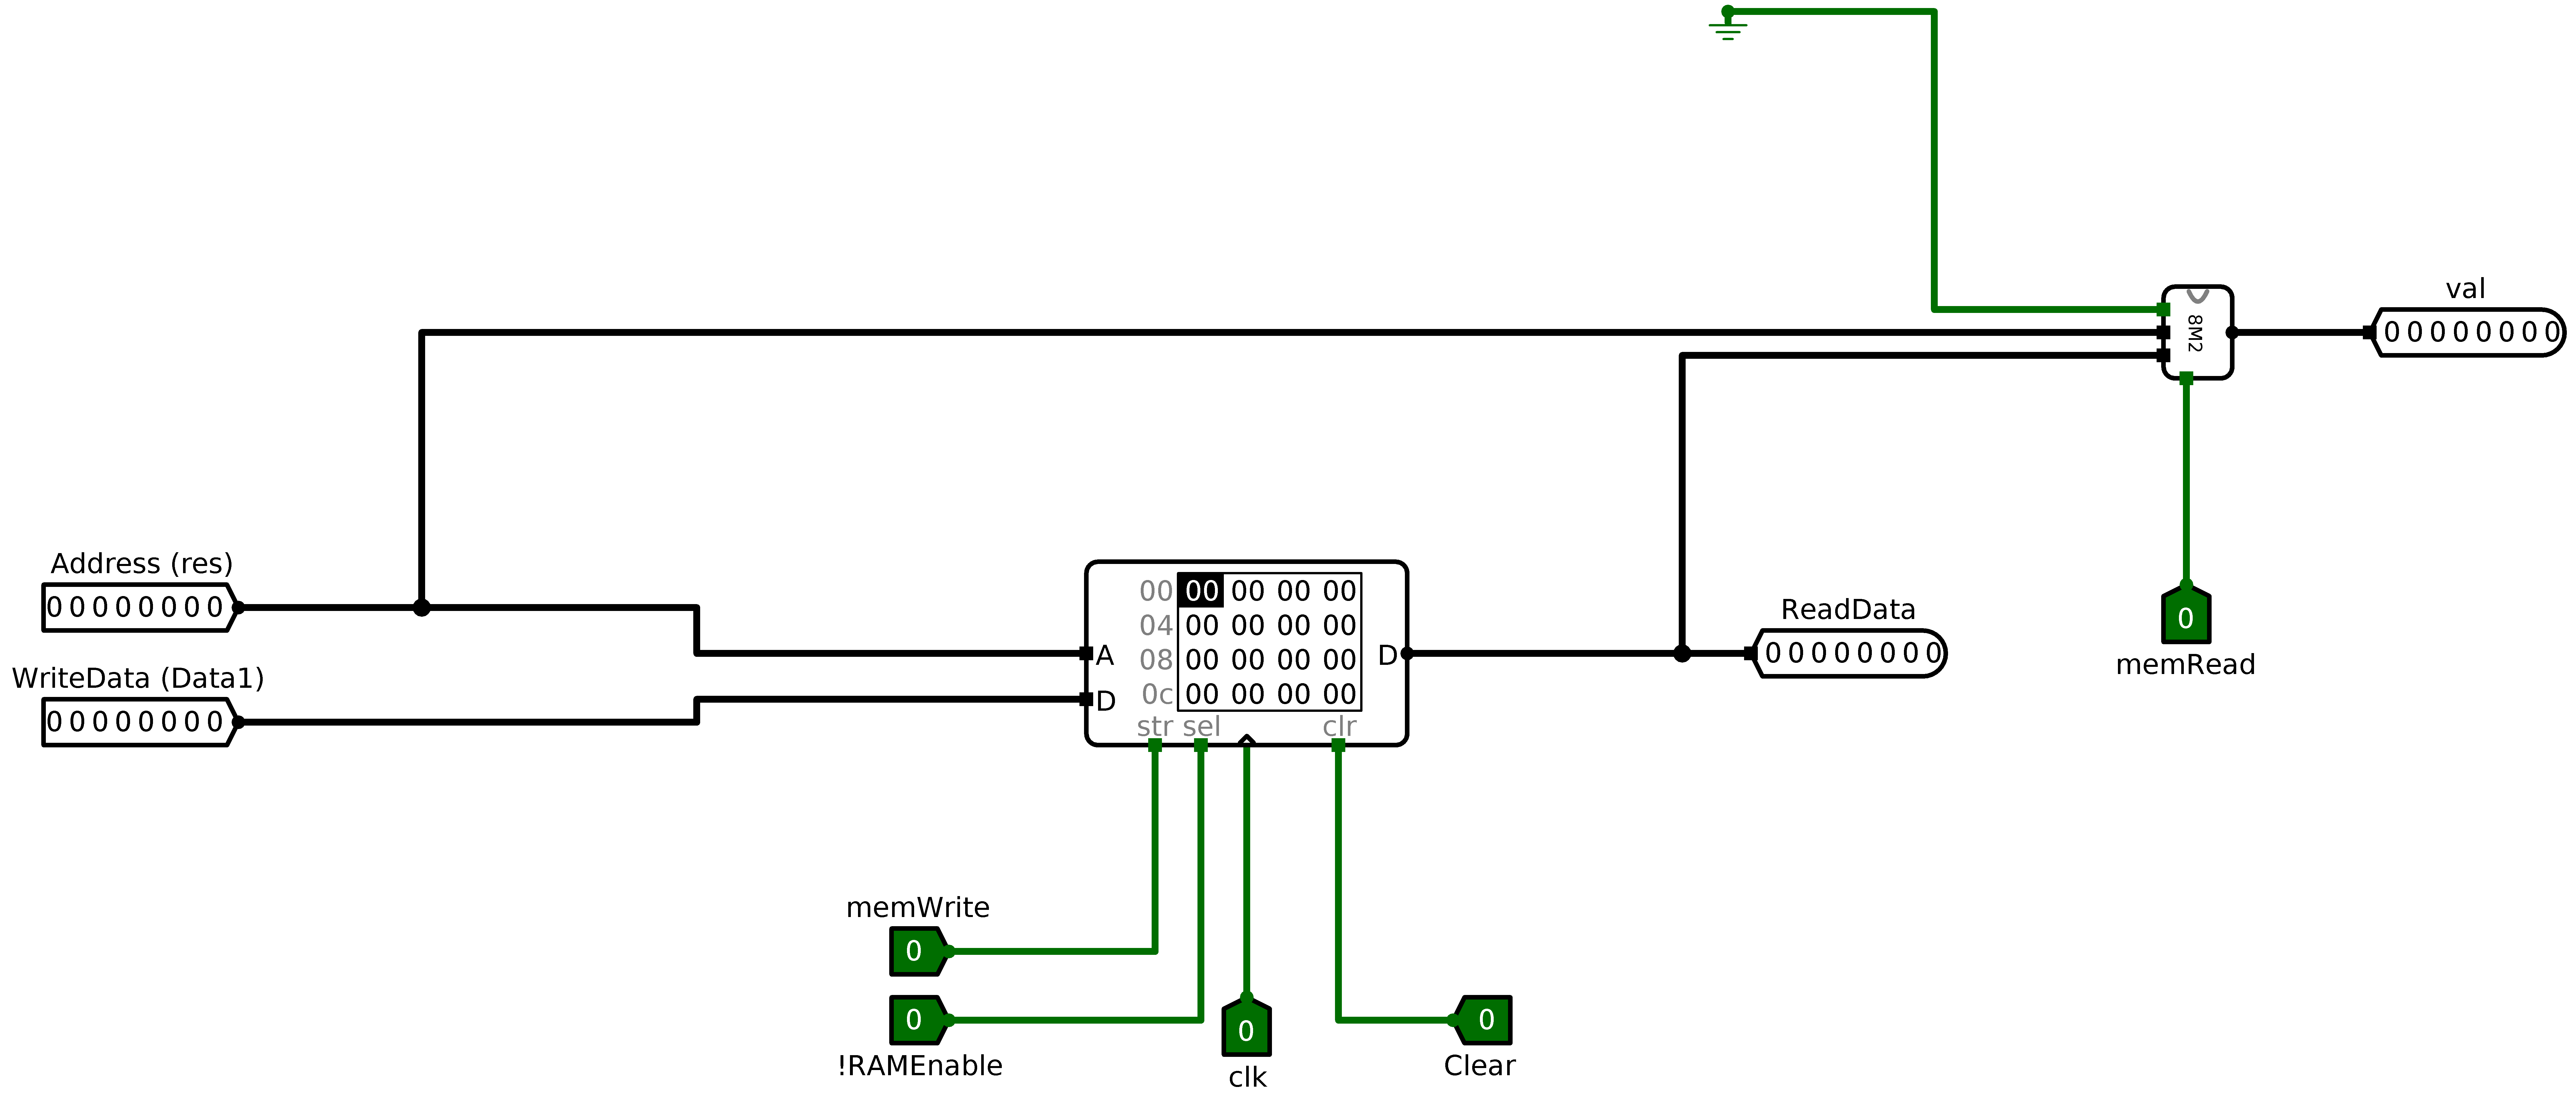
\includegraphics[width=\textwidth]{Images/Memory.png}
     \caption{Memory Unit}
     \label{fig:mem}
 \end{figure}

 \begin{figure}[H]
     \centering
     \includegraphics[width=\textwidth]{Images/MIPS.png}
     \caption{The Complete MIPS}
     \label{fig:mips}
 \end{figure}

\newpage
\section{\large{How to write and execute a program in this machine}}
\label{prog}
Along with implementing the hardware, we have constructed a basic \href{https://github.com/risenfromashes/cse306/tree/ashraf/MIPS/Assembler}{assembler}, which will take a MIPS program and generate machine code instructions in accordance with \hyperref[IS]{Instruction Set}. This instruction needs to be burnt in the instruction memory (In our implementation, an Atmega32). If there are hazards in the program, the assembler will handle that inserting NoOps. For giving clocks, we have two options - automatic (Using Atmega) and manual (Using Push Button).

\newpage
\section{\large{Special Features Implemented}}
\label{Spec}
\subsection{Stack Memory}
We have kept two special registers SP and BP to help in stack operations. SP will point to the top of the stack if not updated manually. BP can be used to support function calling. AT the beginning of the program execution SP and BP will be FF in hexadecimal.
\subsection{8 Bit Data}
We were primarily instructed to build a 4-bit MIPS computer. We have extended our MIPS computer and now it has 8-bit data bus and 8-bit ALU. SO, our computer can operate on larger data.
\subsection{Pipelining}
Pipelining is used in most of the modern architectures. Pipelining improves the performance of a computer significantly. We have implemented a simple version of pipelining in our computer. There are five pipelining stages: Instruction Fetch, Instruction Decode, Execution in ALU, Memory Read or Write, Write Back to Register.
\subsection{Segment for PC}
Our system has 8 bit program counter. But with 8 bit there can be at most 255 instructions in a program. So, we introduced segment register to extend this limit. Our system includes 4 bit segment along with 8 bit PC, so there are total 12 bits for instruction memory addressing. That means there can be at most 4095 instructions which is much larger 
\subsection{Special Instructions}
We have introduced two special instructions along with the instruction set specified. J-type format of our instruction set has four spare bits. These bits can be utilized to introduce extra instructions. We used those spare bits for our special instructions, so bits needed for opcode remains the same. The special instructions are:
\subsubsection{Jump Register}
This instruction will read two registers from the register bank. One will be considered as the new PC and the low 4 bits of the other is the new segment. Then the instruction will jump to that segment and PC. This instruction will help to implement functions. To return from a function to its calling routine, we need this jump register instruction. Format of the instruction: \\
\newline
\vspace{15}
\begin{tabular}{|p{3cm}|p{2cm}|p{4cm}|p{2.5cm}|}
    \hline
     Opcode for j & Src Reg 1 & Src Reg 2 & 4 \\
     \hline
     4 bits & 4 bits & 4 bits & 4 bits \\
     \hline
\end{tabular}
\subsubsection{No Operation}
We have implemented a simple version of pipelining, which is not hazard free. So, we must stall one or two cycles to avoid data corruption if hazard arises. No operation or NoOp can help to stall the pipeline. This instruction blocks the register bank and data memory to write anything. Format of the instruction: \newline
\vspace{15}
\begin{tabular}{|p{3cm}|p{3cm}|p{3cm}|p{2.5cm}|}
    \hline
     Opcode for j & Don't Care & Don't Care & 8 \\
     \hline
     4 bits & 4 bits & 4 bits & 4 bits \\ 
     \hline
\end{tabular}
\subsection{Support for Function Calling}
Our system can support function calling with some help of the assembler. As we have both BP and SP, functions can use them to manipulate local variables. We also have introduced jump register instruction. The assembler needs to save the return address in the stack when a function is called. When the callee function ends execution, it will pop the PC and segment of the return address in two registers. Then, using jump register instruction, the control will be returned to the caller function. Thus, function calling can be supported.

\subsection{Control Forwarding}
As we have implemented pipelining, we might need to flush 3 stages if branch instruction is taken. This is not efficient. So, we have placed this decision in the ID (Instruction Decode) stage. Data from two source registers are compared immediately after they are read. The result of this comparison is used along with control flags and sent to IF(Instruction Fetch) stage. Also control flags for unconditional jump are directly sent to IF stage. For this, at most one flush is needed. SO, this is an improvement. All kind of jumps (Conditional, Unconditional, Register) are directly materialised immediately after ID stage.

\newpage
\section{\large{ICs used with their count}}
\label{IC}
\subsection{Instruction Fetch}
\begin{table}[h]
    \centering
    \begin{tabular}{lc}
    \textbf{IC} & \textbf{Quantity} \\
    \hline \hline
    IC 7483 & 3 \\
    IC 7408 & 1 \\
    IC 7432 & 1 \\    
    IC 74157 & 5 \\    
    IC 7495 & 3 \\
    Atmega32A & 1 \\
    \hline
    Total & 14
\end{tabular}
\end{table}

\subsection{Instruction Decode}
\begin{table}[h]
    \centering
    \begin{tabular}{lc}
    \textbf{IC} & \textbf{Quantity} \\
    \hline \hline
    IC 7408 & 1 \\
    IC 7486 & 1 \\ 
    IC 74157 & 5 \\
    Atmega32A & 2 \\
    \hline
    Total & 9
\end{tabular}

\end{table}
\subsection{Execution}
\begin{table}[h]
    \centering
    \begin{tabular}{lc}
    \textbf{IC} & \textbf{Quantity} \\
    \hline \hline
    IC 74157 & 4 \\
    Atmega32A & 1 \\
    \hline
    Total & 5
\end{tabular}
\end{table}
\subsection{Memory}
\begin{table}[H]
    \centering
    \begin{tabular}{lc}
    \textbf{IC} & \textbf{Quantity} \\
    \hline \hline
    IC 74157 & 2 \\
    Atmega32A & 1 \\
    \hline
    Total & 3
\end{tabular}
\end{table}
\newpage
\subsection{Pipeline Registers}
Number of IC 7495 as Pipeline Registers between different stages \\
\begin{table}[H]
    \centering
    \begin{tabular}{lc}
    \textbf{Stage} & \textbf{Quantity} \\
    \hline \hline
    IF-ID & 5 \\
    ID-EX & 8 \\
    EX-MEM & 6 \\
    MEM-RW & 4 \\
    \hline
    Total & 23
\end{tabular}
\end{table}

\subsection{Total}
\begin{table}[h]
    \centering
    \begin{tabular}{lc}
    \textbf{IC} & \textbf{Quantity} \\
    \hline \hline
    IC 7483 & 3 \\
    IC 7408 & 2 \\
    IC 7432 & 1 \\    
    IC 7486 & 1 \\
    IC 74157 & 16 \\    
    IC 7495 & 26 \\
    Atmega32A & 6 \\
    \hline
    Total & 55
\end{tabular}
\end{table}

\newpage
\section{\large{Discussion}}
In this lab report, we discuss our implementation of an 8-bit MIPS PC with pipelining, which goes beyond the initial requirements of the project that called for a 4-bit MIPS PC in both hardware and software. While we acknowledge that our implementation exceeds the original scope, we believe that the additional complexity and features add value to our project and provide a more comprehensive understanding of the MIPS architecture and its implementation.\\

The fact that an 8-bit PC allows for a wider range of memory addresses, which can be useful in more complex programs inspired us to go for it. More wires made the circuit more complex, also debugging was more difficult for this. We also faced the challenge of running out of available pins on a ATmega microcontroller in Instruction Decode Stage. To address this issue, we utilized another ATmega and used USART (Universal Synchronous/Asynchronous Receiver/Transmitter) communication between these two. This allowed us to transfer data and instructions between the two microcontrollers, freeing up additional pins for other functions. The USART communication was implemented using the UART protocol, which provided a reliable and efficient means of transmitting data between the two microcontrollers. This introduction allowed us to overcome the hardware limitations and successfully implement our 8-bit MIPS PC with pipelining. \\

Pipelining is a widely used technique in modern processors and plays a critical role in improving their performance. We decided to introduce it in our hardware despite it being a daunting task. Implementing pipelining in our MIPS PC project posed several challenges. One of the primary challenges was to properly incorporate the Parallel In Parallel Out (PIPO) registers. We had to rigorously test a significant amount of these registers to obtain enough ones for our implementation. Managing so many of them and ensuring proper data flow in between the stages was indeed a challenge. Pipelining also introduced new complexities in debugging and testing the processor design. However, regardless of these challenges, implementing pipelining was a valuable learning experience that enhanced our knowledge of processor architecture and design.\\


Overall, we believe that our pipelined 8-bit MIPS PC adds value to our project and provides a more comprehensive understanding of the MIPS architecture and its implementation.
\end{document}